\documentclass[a4paper,12pt]{article}
\usepackage[latin1]{inputenc}
\usepackage[spanish]{babel}
\usepackage{bm}
\usepackage{graphicx}
\usepackage{amsmath}
\usepackage{enumerate}
%\documentstyle[12pt,bezier]{articulo}
\setlength{\textheight}{235mm}
\setlength{\textwidth}{168mm}
\setlength{\oddsidemargin}{0pt}
\pagestyle{empty}

\begin{document}
\mbox{}\vspace*{-45mm}

{\centering
{\small\sc Escuela T�cnica Superior de Ingenieros de Caminos, Canales y
Puertos (Madrid)}\\*[4mm]
{\Large\bf M�todo de los Elementos Finitos}\\*[4mm]
EJERCICIO 2: Modelos de potencial \\*[4mm]
}
%%%%%
\noindent
La figura adjunta representa una pantalla pr�cticamente impermeable, construida
sobre un terreno cuya permeabilidad es $k=8.5\cdot 10^{-5}$ m/s.
Para los niveles de agua indicados en dicha figura se desean analizar los  valores de las filtraciones. Se supone que los bordes verticales est�n lo suficientemente alejados de la pantalla como para que no afecten a las filtraciones bajo la misma (el flujo a trav�s de ellos se puede considerar nulo).

{\em En el mallado se utilizar�n elementos cuadril�teros de $4$ nodos. Para generar la malla de elementos finitos el tama�o global aproximado se tomar� igual a
$1.4$ m.}
\begin{center}
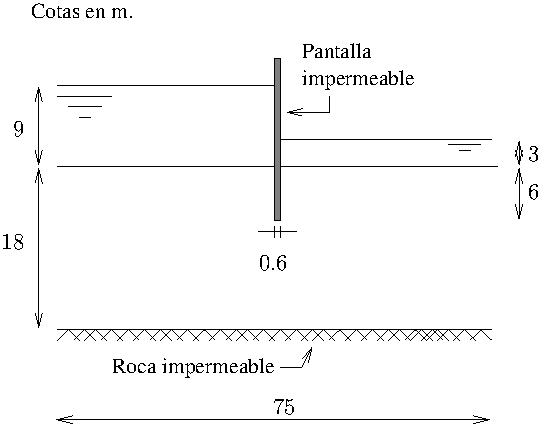
\includegraphics[width=0.7\textwidth]{ejercici2}
\end{center}
\end{document}
